\section{Sideband Transitions}
\label{sec:sideband_transition}

%We aim to characterize the interaction between a two-level system and light, a task typically accomplished using the well-known Jaynes-Cummings Hamiltonian \cite{haroche2006exploring}.
%This model enables us to implement two-qubit gates, as the interaction between the two qubits causes their energy levels to hybridize.
%By appropriately manipulating the signal sent to the tunable couplers, we can regulate this interaction and thus execute specific gates. 

We aim to characterize the interaction between two distinct two-level systems, with the goal of inducing Rabi oscillations between their energy levels.
These systems belongs to separate qubits, thus the two-level systems are off-resonant.
This two-level manifold in which excitations are passed between two qubits are known as \emph{sideband transition}.

To achieve Rabi oscillations on these sideband transitions, we send an AC flux signal directed at a tunable coupler controlling the interaction between the qubits.
This signal is carefully tuned to be on-resonant with the sideband transition.
The resulting two-qubit gates, executed using this approach, are called \emph{parametric gates}.

However, to determine the optimal signal for manipulation, we require accurate parameters from the theoretical model.
Hence, our initial step involves calibrating the interaction between the two levels.

In this section, we present the theoretical framework of the two sideband transitions used in our experiments, essential for fine-tuning the two-qubit gates.

\subsection{Damping-free Regime}

The initial scenario occurs in the absence of any damping or decay within the model.
In this regime, we aim to characterize the sidebands resulting from the hybridization of the energy levels of the two storage qubits.
This situation precisely reflects the interaction between a two-level system and a coherent light field, described by the Hamiltonian modelling the interaction between a two-level atom and a classical light field, in the rotating wave approximation \cite{RWA}
\begin{equation}
    \hat{H} = \hbar
    \begin{pmatrix}
        \omega_{\ket{a}} & g_0           \\
        g_0            & \omega_{\ket{b}}
    \end{pmatrix} ,
\end{equation}
where $\omega_{\ket{a}}$ and $\omega_{\ket{b}}$ are the frequency of the first and second energy level, respectively.
In the specific scenario under consideration, these levels will manifest as sidebands.
However, for the sake of generality, we choose to maintain a more general labeling scheme.
The parameter $g_0$ represents the coupling strength between the two levels, a quantity that can be adjusted via the SQUID loop incorporated within the tunable couplers connecting the qubits.

If we shift the energy by $\omega_{\ket{a}}$, define the detuning $\omega_{ab} = \omega_{\ket{b}} - \omega_{\ket{a}}$ between the two levels and move in the frame rotating with the drive at its frequency $\omega$, we get
\begin{equation}
\label{eq:JC-Chevron}
    \hat{H} = \hbar
    \begin{pmatrix}
        0       & g_0       \\
        g_0   & \delta  
    \end{pmatrix},
\end{equation}
where $\delta = \omega_{ab} - \omega$.

%Following from the Schrödinger equation, the time volution of an arbitrary state is given by 
%\begin{equation}
%    \ket{\psi ( t )} = \hat{U}(t) \ket{\psi(0)} ,
%\end{equation}
%where $\hat{U}(t)$ is the unitary evolution of the Hamiltonian
%\begin{equation}
%    \hat{U}(t) = e^{-i \hat{H} t / \hbar} .
%\end{equation}

If the initial state is $\ket{a}$, the time evolution of the population obtained with Schrödinger's equation with this Hamiltonian is given by \cite{Lacroix}
\begin{equation}
\label{eq:chevron}
    P_{\ket{a}} (t) = \Tr \left( \hat{U}(t) \ket{a} \bra{a} \hat{U}^\dagger (t) \right) = 
    \frac{\delta^2 + 2 g_0^2 
    \left( \cos(\sqrt{4 g_0^2 + \delta^2} t) + 1 \right)}{4 g_0^2 + \delta^2} ,
\end{equation}
with a period of $2 \pi / \Omega$, where $\Omega$ is the \emph{effective Rabi frequency}.
This latter is defined as
\begin{equation}
    \Omega = \sqrt{4 g_0^2 + \delta^2} .
\end{equation}

The population as a function of time $t$ and detuning $\delta$ results in a Chevron pattern, shown in \cref{fig:Chevron}.

\begin{figure}
    \centering
    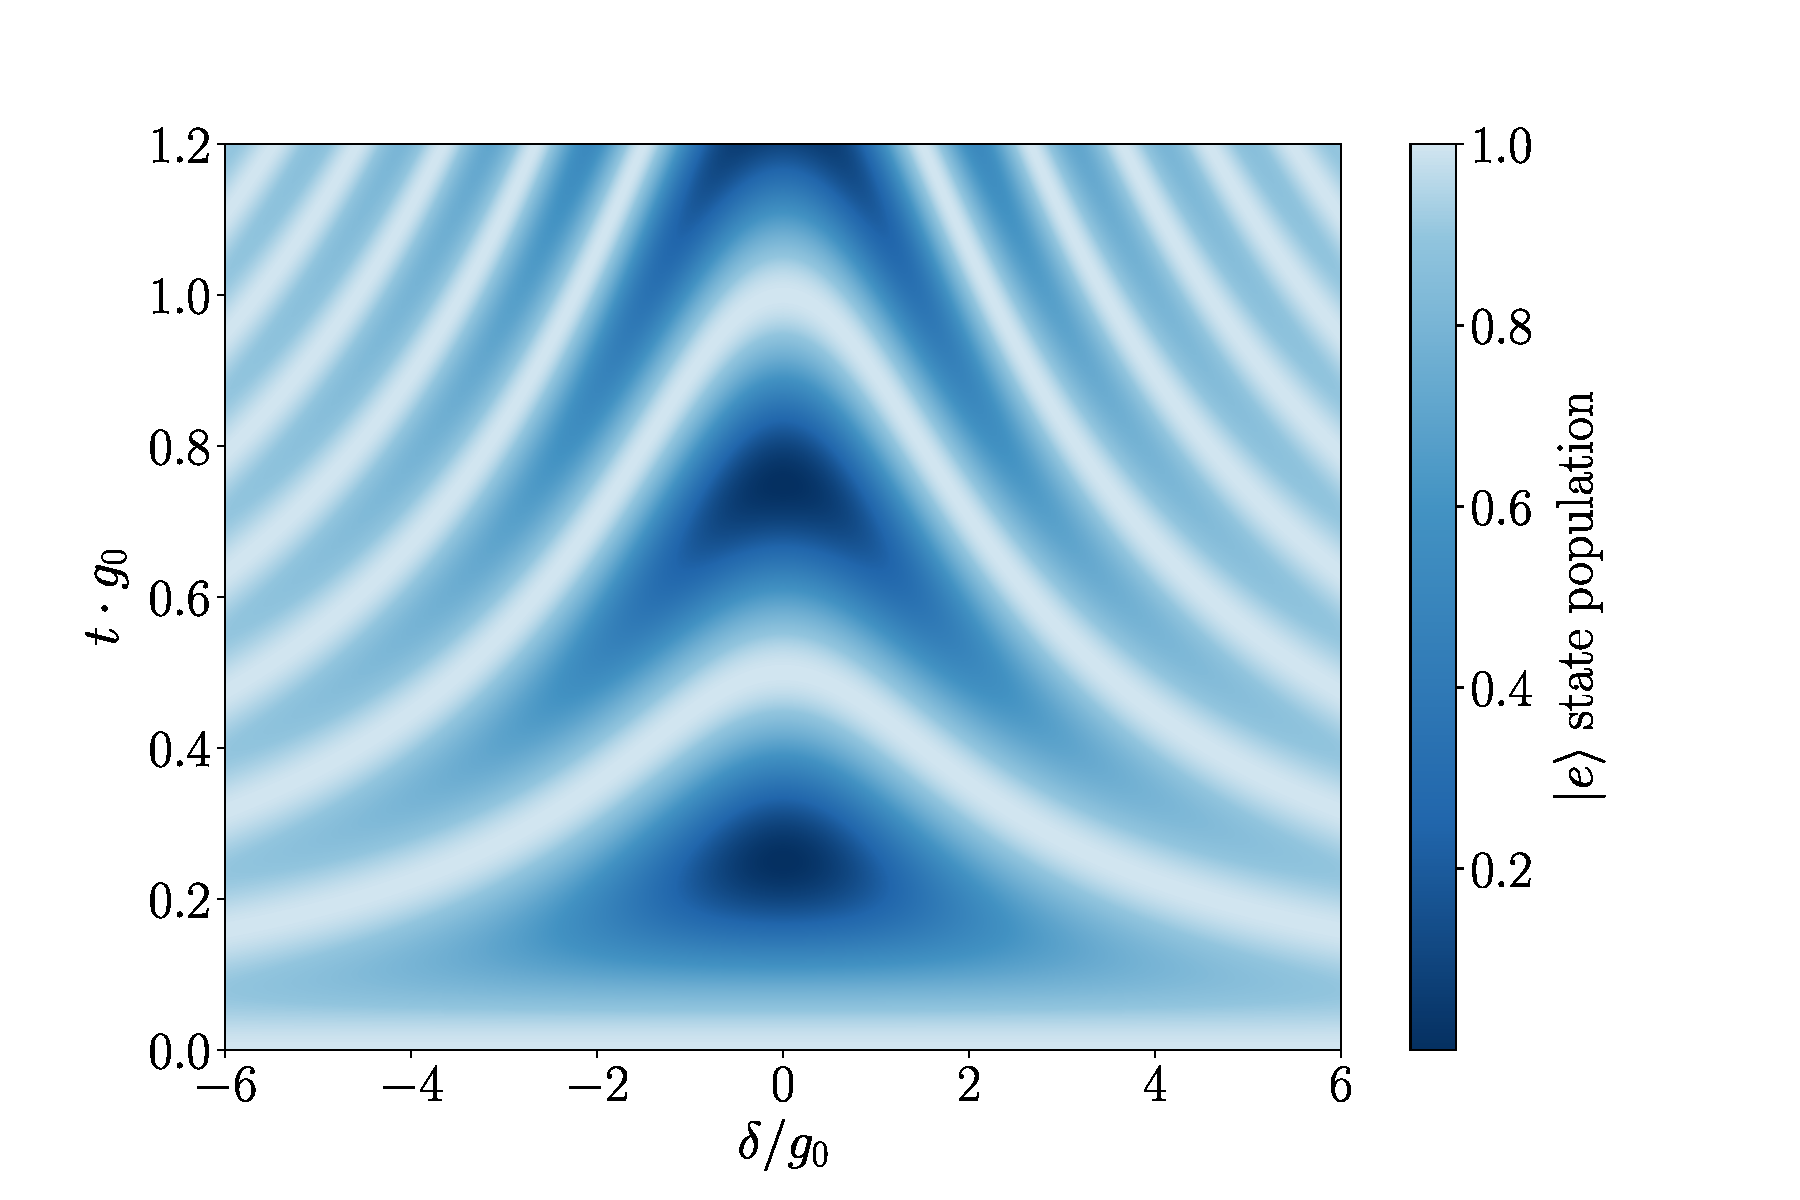
\includegraphics[width = 0.8\textwidth]{Images/Chap3/Chevron.pdf}
    \caption{Chevron pattern arising from \cref{eq:chevron}}
    \label{fig:Chevron}
\end{figure}

In our experimental setup, we employ the model outlined in \cref{eq:chevron} to fine-tune the interaction between storage elements. 
We collect data as a function of both the detuning $\delta$ between the sideband energy levels and the interaction time $t$. 
This approach allows us to determine the model parameters effectively, thus finding the operational configuration required for implementing the desired gate.

\subsection{Damped Regime}

\begin{figure}
    \centering
    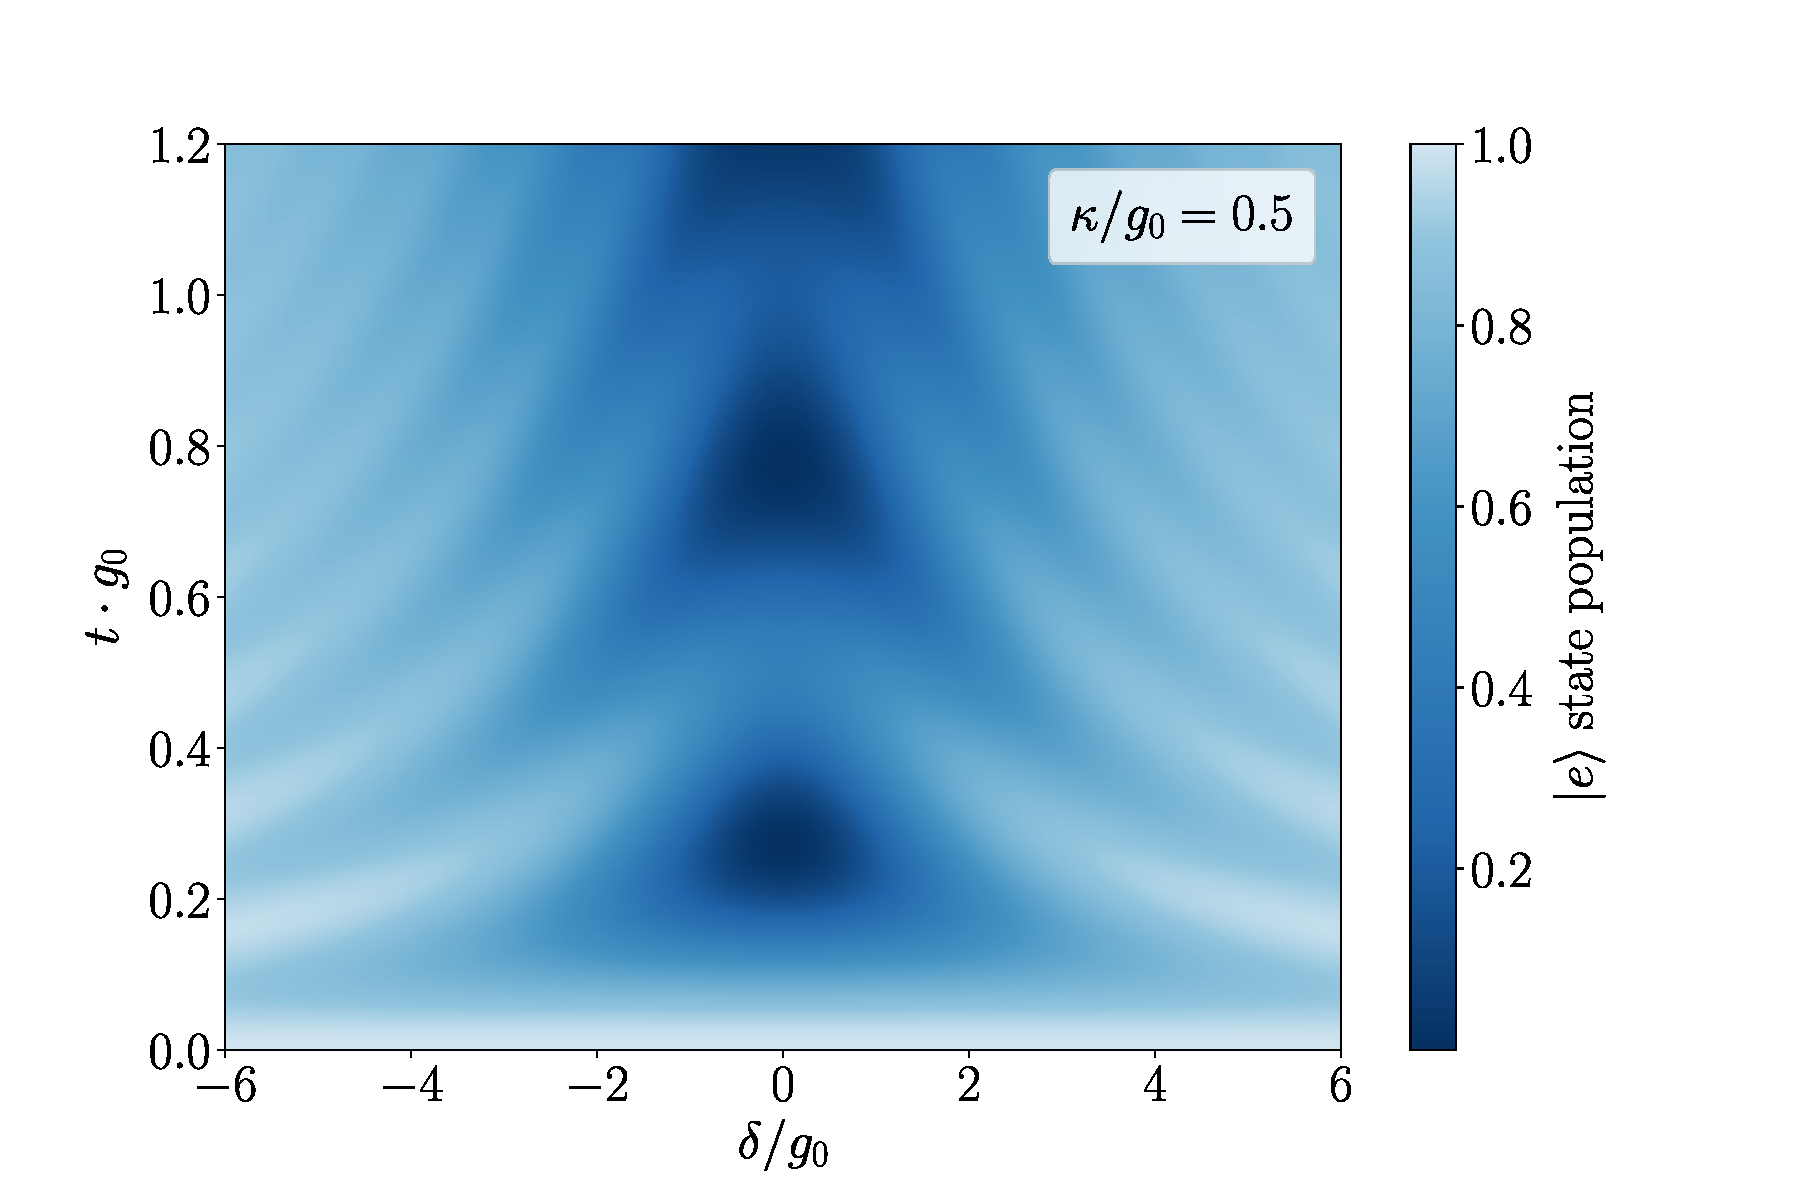
\includegraphics[width = 0.8\textwidth]{Images/Chap3/Chevron_kappa.pdf}
    \caption{Damped regime of the Chevron arising from \cref{eq:chevron_kappa}}
    \label{fig:chevron_kappa}
\end{figure}

To properly model the interaction between the storage and emitter, it is essential to take into account the strong coupling of the emitter qubit to the emission line. 
Consequently, we must consider the decay of excitation into photons emitted through the emission line. 

A practical approach to incorporate this external loss is by considering \cref{eq:JC-Chevron} with an additional non-Hermitian term, $-i \kappa \ket{a} \bra{a} / 2$ \cite{Magnard2021}.
We can write the new Hamiltonian as
\begin{equation}
\label{eq:JC-decay}
    \hat{H} = \hbar
    \begin{pmatrix}
        0       & g_0       \\
        g_0   & \delta - i \frac{\kappa}{2} 
    \end{pmatrix}  .
\end{equation}

By diagonalizing the Hamiltonian
\begin{equation}
    \hat{H} = S \hat{D} S^{-1} ,
\end{equation}
we can employ a similar approach as before to find the time evolution of the system
\begin{equation}
    \ket{\psi (t)} = e^{-i \hat{H} t / \hbar} \ket{\psi(0)}= 
    S e^{-i \hat{D} t / \hbar} S^{-1} \ket{\psi(0)} .
\end{equation}
If $\ket{\psi(0)} = \ket{g}$, then the time evolution of the population of the ground state is
\begin{equation}
\label{eq:chevron_kappa}
    P_{\ket{g}} (t) = 
\left| \cos \left(\frac{\Omega t}{2} \right) + \frac{\delta - i \kappa / 2}{\Omega} \sin \left(\frac{\Omega t}{2} \right) \right|^2 e^{- \frac{\kappa t}{2}} .
\end{equation}
Here, the effective Rabi frequency is defined as
\begin{equation}
\label{eq:eff_Raby_kappa}
    \Omega = \sqrt{4 g_0^2 + \left( \delta - i \kappa / 2 \right)^2} .
\end{equation}
The main difference with respect to \cref{eq:chevron} is the presence of the exponential decay $e^{-kt/2}$.

The plot of the population as a function of the detuning $\delta$ and of time $t$ is shown in \cref{fig:chevron_kappa}.
The value of the decay parameter used is $\kappa / g_0 = 0.5$.